
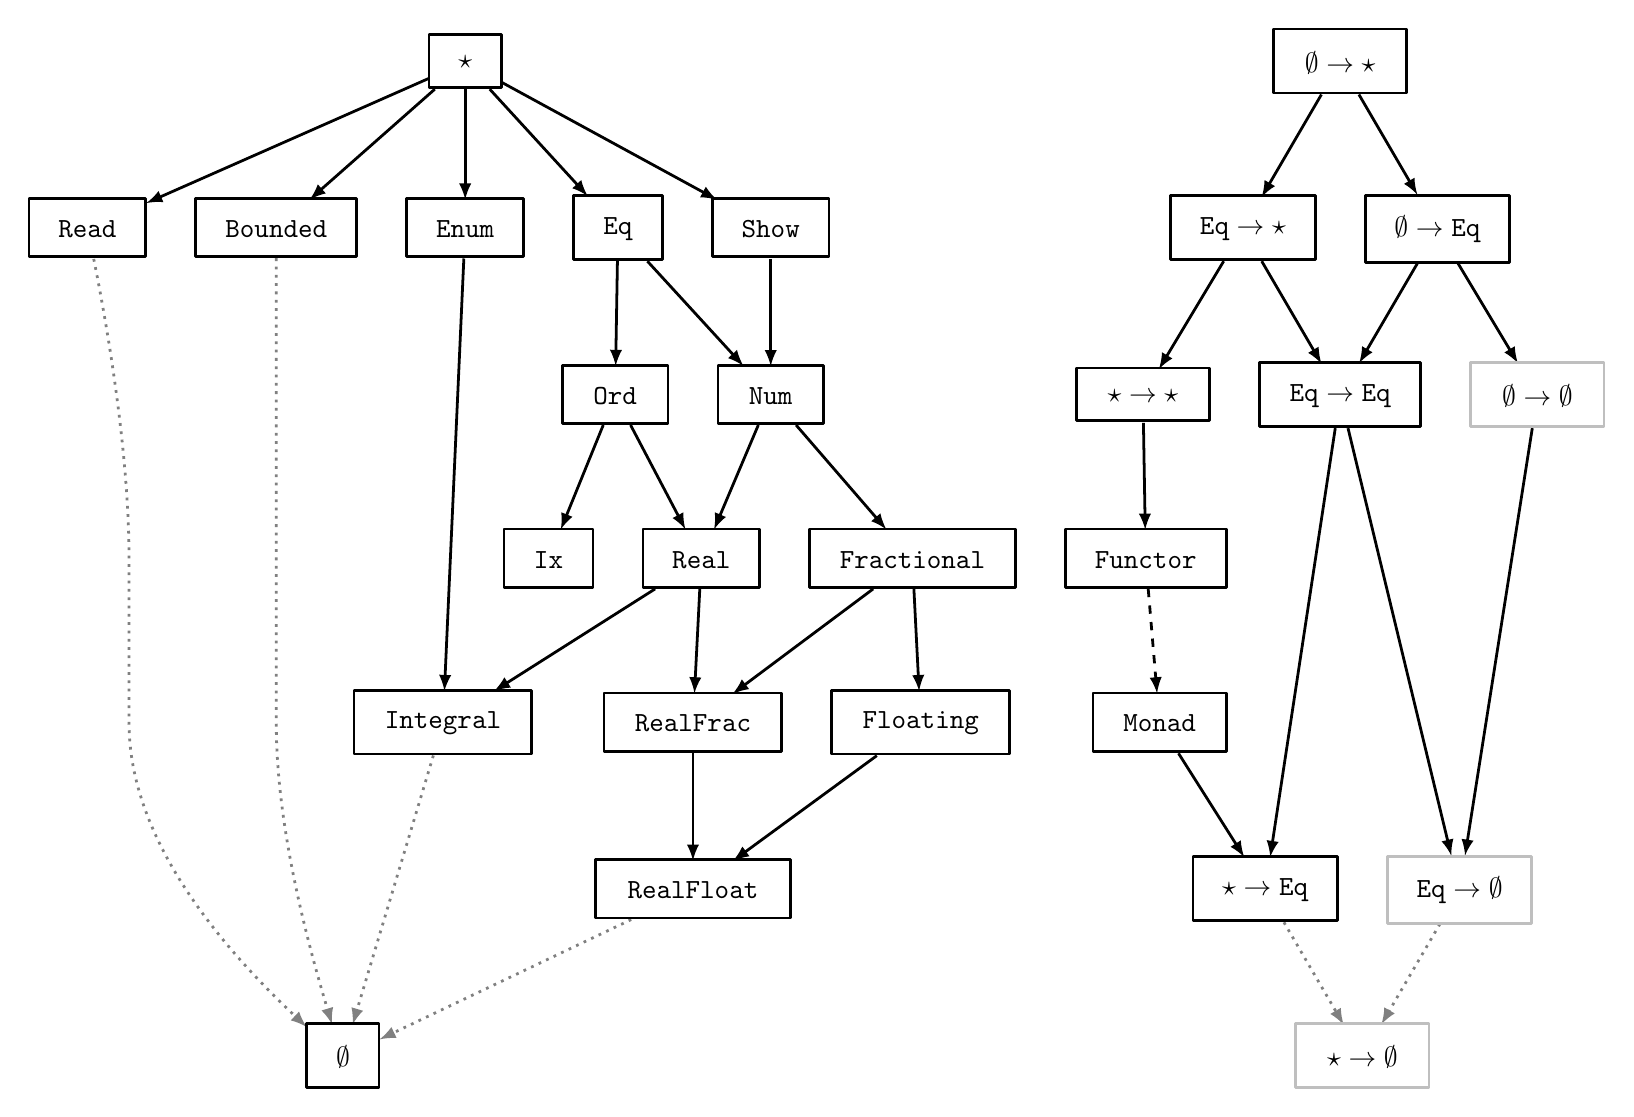
\begin{tikzpicture}[>=latex,line join=bevel,]
  \pgfsetlinewidth{1bp}
%%
\pgfsetcolor{black}
  % Edge: \texttt{Eq} -> \texttt{Num}
  \draw [->] (222.6bp,298.43bp) .. controls (230.41bp,289.92bp) and (241.18bp,278.17bp)  .. (257.17bp,260.73bp);
  % Edge: \texttt{Show} -> \texttt{Num}
  \draw [->] (267bp,299.27bp) .. controls (267bp,291.34bp) and (267bp,280.28bp)  .. (267bp,260.63bp);
  % Edge: \emptyset \to \emptyset -> \texttt{Eq} \to \emptyset
  \draw [->] (541.16bp,238.32bp) .. controls (536.58bp,209.18bp) and (524.57bp,132.85bp)  .. (516.95bp,84.428bp);
  % Edge: \texttt{Floating} -> \texttt{RealFloat}
  \draw [->] (305.19bp,120.43bp) .. controls (292.78bp,111.35bp) and (275.34bp,98.592bp)  .. (253.39bp,82.528bp);
  % Edge: \star \to \texttt{Eq} -> \star \to \emptyset
  \pgfsetcolor{gray}
  \draw [->,dotted] (451.75bp,60.431bp) .. controls (456.4bp,52.463bp) and (462.7bp,41.662bp)  .. (473.27bp,23.533bp);
  % Edge: \texttt{RealFloat} -> \emptyset
  \draw [->,dotted] (216.76bp,61.411bp) .. controls (193.87bp,50.51bp) and (158.39bp,33.615bp)  .. (126.14bp,18.256bp);
  % Edge: \texttt{Ord} -> \texttt{Ix}
  \pgfsetcolor{black}
  \draw [->] (206.71bp,239.45bp) .. controls (203.54bp,231.66bp) and (199.13bp,220.82bp)  .. (191.42bp,201.86bp);
  % Edge: \emptyset \to \star -> \texttt{Eq} \to \star
  \draw [->] (465.25bp,358.43bp) .. controls (460.6bp,350.46bp) and (454.3bp,339.66bp)  .. (443.73bp,321.53bp);
  % Edge: \texttt{Fractional} -> \texttt{Floating}
  \draw [->] (318.54bp,180.45bp) .. controls (318.91bp,173.02bp) and (319.43bp,162.8bp)  .. (320.41bp,143.67bp);
  % Edge: \texttt{Num} -> \texttt{Fractional}
  \draw [->] (276.12bp,239.45bp) .. controls (283.28bp,231.17bp) and (293.43bp,219.42bp)  .. (308.62bp,201.86bp);
  % Edge: \star -> \texttt{Bounded}
  \draw [->] (146.07bp,360.36bp) .. controls (136.07bp,351.53bp) and (121.02bp,338.25bp)  .. (101.04bp,320.63bp);
  % Edge: \emptyset \to \texttt{Eq} -> \emptyset \to \emptyset
  \draw [->] (514.29bp,297.86bp) .. controls (518.98bp,290.03bp) and (525.21bp,279.65bp)  .. (535.97bp,261.72bp);
  % Edge: \emptyset \to \star -> \emptyset \to \texttt{Eq}
  \draw [->] (478.75bp,358.43bp) .. controls (483.28bp,350.67bp) and (489.38bp,340.21bp)  .. (499.79bp,322.36bp);
  % Edge: \star \to \star -> \texttt{\texttt{Functor}}
  \draw [->] (401.17bp,240.26bp) .. controls (401.3bp,232.55bp) and (401.48bp,221.52bp)  .. (401.82bp,201.76bp);
  % Edge: \texttt{\texttt{Monad}} -> \star \to \texttt{Eq}
  \draw [->] (413.79bp,121.27bp) .. controls (418.84bp,113.3bp) and (425.88bp,102.19bp)  .. (437.48bp,83.868bp);
  % Edge: \texttt{Real} -> \texttt{Integral}
  \draw [->] (225.37bp,180.45bp) .. controls (211.75bp,171.81bp) and (192.19bp,159.4bp)  .. (167.39bp,143.67bp);
  % Edge: \texttt{Read} -> \emptyset
  \pgfsetcolor{gray}
  \draw [->,dotted] (23.278bp,299.23bp) .. controls (27.474bp,278.42bp) and (36bp,231.19bp)  .. (36bp,191bp) .. controls (36bp,191bp) and (36bp,191bp)  .. (36bp,132bp) .. controls (36bp,90.15bp) and (69.583bp,51.239bp)  .. (99.938bp,22.743bp);
  % Edge: \texttt{Enum} -> \texttt{Integral}
  \pgfsetcolor{black}
  \draw [->] (156.52bp,299.4bp) .. controls (155.24bp,270.92bp) and (151.71bp,192.34bp)  .. (149.53bp,143.69bp);
  % Edge: \texttt{Bounded} -> \emptyset
  \pgfsetcolor{gray}
  \draw [->,dotted] (89bp,299.49bp) .. controls (89bp,278.75bp) and (89bp,231.08bp)  .. (89bp,191bp) .. controls (89bp,191bp) and (89bp,191bp)  .. (89bp,132bp) .. controls (89bp,96.994bp) and (98.942bp,57.34bp)  .. (109.04bp,23.766bp);
  % Edge: \texttt{Eq} \to \emptyset -> \star \to \emptyset
  \draw [->,dotted] (507.92bp,59.858bp) .. controls (503.35bp,52.03bp) and (497.3bp,41.653bp)  .. (486.83bp,23.715bp);
  % Edge: \star -> \texttt{Enum}
  \pgfsetcolor{black}
  \draw [->] (157bp,360.36bp) .. controls (157bp,352.38bp) and (157bp,340.76bp)  .. (157bp,320.63bp);
  % Edge: \star -> \texttt{Read}
  \draw [->] (143.96bp,364.25bp) .. controls (122.81bp,354.92bp) and (80.493bp,336.25bp)  .. (42.178bp,319.34bp);
  % Edge: \texttt{Eq} \to \texttt{Eq} -> \texttt{Eq} \to \emptyset
  \draw [->] (474.82bp,238.32bp) .. controls (481.86bp,209.18bp) and (500.3bp,132.85bp)  .. (512bp,84.428bp);
  % Edge: \texttt{Eq} -> \texttt{Ord}
  \draw [->] (211.81bp,298.43bp) .. controls (211.68bp,290.6bp) and (211.5bp,280.03bp)  .. (211.18bp,260.73bp);
  % Edge: \star -> \texttt{Show}
  \draw [->] (170.05bp,362.88bp) .. controls (186.88bp,353.7bp) and (216.62bp,337.48bp)  .. (247.68bp,320.54bp);
  % Edge: \texttt{Eq} \to \star -> \texttt{Eq} \to \texttt{Eq}
  \draw [->] (443.75bp,298.43bp) .. controls (448.4bp,290.46bp) and (454.7bp,279.66bp)  .. (465.27bp,261.53bp);
  % Edge: \texttt{Ord} -> \texttt{Real}
  \draw [->] (216.54bp,239.45bp) .. controls (220.72bp,231.5bp) and (226.58bp,220.35bp)  .. (236.3bp,201.86bp);
  % Edge: \texttt{Num} -> \texttt{Real}
  \draw [->] (262.53bp,239.45bp) .. controls (259.23bp,231.66bp) and (254.63bp,220.82bp)  .. (246.6bp,201.86bp);
  % Edge: \texttt{Fractional} -> \texttt{RealFrac}
  \draw [->] (303.88bp,180.45bp) .. controls (292.15bp,171.7bp) and (275.26bp,159.08bp)  .. (253.27bp,142.66bp);
  % Edge: \texttt{Eq} \to \texttt{Eq} -> \star \to \texttt{Eq}
  \draw [->] (470.23bp,238.32bp) .. controls (465.79bp,209.04bp) and (454.12bp,132.11bp)  .. (446.81bp,83.955bp);
  % Edge: \texttt{Real} -> \texttt{RealFrac}
  \draw [->] (241.46bp,180.45bp) .. controls (241.08bp,172.83bp) and (240.54bp,162.28bp)  .. (239.55bp,142.86bp);
  % Edge: \texttt{Integral} -> \emptyset
  \pgfsetcolor{gray}
  \draw [->,dotted] (145.55bp,120.49bp) .. controls (139.54bp,100.48bp) and (127.08bp,58.946bp)  .. (116.49bp,23.648bp);
  % Edge: \emptyset \to \texttt{Eq} -> \texttt{Eq} \to \texttt{Eq}
  \pgfsetcolor{black}
  \draw [->] (499.92bp,297.86bp) .. controls (495.35bp,290.03bp) and (489.3bp,279.65bp)  .. (478.83bp,261.72bp);
  % Edge: \texttt{RealFrac} -> \texttt{RealFloat}
  \draw [->] (239bp,121.27bp) .. controls (239bp,113.34bp) and (239bp,102.28bp)  .. (239bp,82.634bp);
  % Edge: \star -> \texttt{Eq}
  \draw [->] (165.84bp,360.36bp) .. controls (173.48bp,352.02bp) and (184.77bp,339.7bp)  .. (201.1bp,321.89bp);
  % Edge: \texttt{\texttt{Functor}} -> \texttt{\texttt{Monad}}
  \draw [->,dashed] (402.89bp,180.45bp) .. controls (403.54bp,172.83bp) and (404.43bp,162.28bp)  .. (406.08bp,142.86bp);
  % Edge: \texttt{Eq} \to \star -> \star \to \star
  \draw [->] (430.06bp,298.43bp) .. controls (424.92bp,289.86bp) and (417.81bp,278.02bp)  .. (406.73bp,259.56bp);
  % Node: \texttt{Show}
\begin{scope}
  \definecolor{strokecol}{rgb}{0.0,0.0,0.0};
  \pgfsetstrokecolor{strokecol}
  \draw (288bp,321bp) -- (246bp,321bp) -- (246bp,300bp) -- (288bp,300bp) -- cycle;
  \draw (267bp,310bp) node {$\texttt{Show}$};
\end{scope}
  % Node: \texttt{Enum}
\begin{scope}
  \definecolor{strokecol}{rgb}{0.0,0.0,0.0};
  \pgfsetstrokecolor{strokecol}
  \draw (178bp,321bp) -- (136bp,321bp) -- (136bp,300bp) -- (178bp,300bp) -- cycle;
  \draw (157bp,310bp) node {$\texttt{Enum}$};
\end{scope}
  % Node: \texttt{Ix}
\begin{scope}
  \definecolor{strokecol}{rgb}{0.0,0.0,0.0};
  \pgfsetstrokecolor{strokecol}
  \draw (203bp,202bp) -- (171bp,202bp) -- (171bp,181bp) -- (203bp,181bp) -- cycle;
  \draw (187bp,191bp) node {$\texttt{Ix}$};
\end{scope}
  % Node: \star
\begin{scope}
  \definecolor{strokecol}{rgb}{0.0,0.0,0.0};
  \pgfsetstrokecolor{strokecol}
  \draw (170bp,380bp) -- (144bp,380bp) -- (144bp,361bp) -- (170bp,361bp) -- cycle;
  \draw (157bp,370bp) node {$\star$};
\end{scope}
  % Node: \texttt{Eq} \to \texttt{Eq}
\begin{scope}
  \definecolor{strokecol}{rgb}{0.0,0.0,0.0};
  \pgfsetstrokecolor{strokecol}
  \draw (501bp,262bp) -- (443bp,262bp) -- (443bp,239bp) -- (501bp,239bp) -- cycle;
  \draw (472bp,250bp) node {$\texttt{Eq} \to \texttt{Eq}$};
\end{scope}
  % Node: \texttt{\texttt{Functor}}
\begin{scope}
  \definecolor{strokecol}{rgb}{0.0,0.0,0.0};
  \pgfsetstrokecolor{strokecol}
  \draw (431bp,202bp) -- (373bp,202bp) -- (373bp,181bp) -- (431bp,181bp) -- cycle;
  \draw (402bp,191bp) node {$\texttt{\texttt{Functor}}$};
\end{scope}
  % Node: \texttt{Bounded}
\begin{scope}
  \definecolor{strokecol}{rgb}{0.0,0.0,0.0};
  \pgfsetstrokecolor{strokecol}
  \draw (118bp,321bp) -- (60bp,321bp) -- (60bp,300bp) -- (118bp,300bp) -- cycle;
  \draw (89bp,310bp) node {$\texttt{Bounded}$};
\end{scope}
  % Node: \texttt{\texttt{Monad}}
\begin{scope}
  \definecolor{strokecol}{rgb}{0.0,0.0,0.0};
  \pgfsetstrokecolor{strokecol}
  \draw (431bp,143bp) -- (383bp,143bp) -- (383bp,122bp) -- (431bp,122bp) -- cycle;
  \draw (407bp,132bp) node {$\texttt{\texttt{Monad}}$};
\end{scope}
  % Node: \texttt{RealFrac}
\begin{scope}
  \definecolor{strokecol}{rgb}{0.0,0.0,0.0};
  \pgfsetstrokecolor{strokecol}
  \draw (271bp,143bp) -- (207bp,143bp) -- (207bp,122bp) -- (271bp,122bp) -- cycle;
  \draw (239bp,132bp) node {$\texttt{RealFrac}$};
\end{scope}
  % Node: \texttt{Fractional}
\begin{scope}
  \definecolor{strokecol}{rgb}{0.0,0.0,0.0};
  \pgfsetstrokecolor{strokecol}
  \draw (355bp,202bp) -- (281bp,202bp) -- (281bp,181bp) -- (355bp,181bp) -- cycle;
  \draw (318bp,191bp) node {$\texttt{Fractional}$};
\end{scope}
  % Node: \texttt{Floating}
\begin{scope}
  \definecolor{strokecol}{rgb}{0.0,0.0,0.0};
  \pgfsetstrokecolor{strokecol}
  \draw (353bp,144bp) -- (289bp,144bp) -- (289bp,121bp) -- (353bp,121bp) -- cycle;
  \draw (321bp,132bp) node {$\texttt{Floating}$};
\end{scope}
  % Node: \texttt{Eq}
\begin{scope}
  \definecolor{strokecol}{rgb}{0.0,0.0,0.0};
  \pgfsetstrokecolor{strokecol}
  \draw (228bp,322bp) -- (196bp,322bp) -- (196bp,299bp) -- (228bp,299bp) -- cycle;
  \draw (212bp,310bp) node {$\texttt{Eq}$};
\end{scope}
  % Node: \star \to \emptyset
\begin{scope}
  \definecolor{strokecol}{rgb}{0.75,0.75,0.75};
  \pgfsetstrokecolor{strokecol}
  \draw (504bp,24bp) -- (456bp,24bp) -- (456bp,1bp) -- (504bp,1bp) -- cycle;
  \definecolor{strokecol}{rgb}{0.0,0.0,0.0};
  \pgfsetstrokecolor{strokecol}
  \draw (480bp,12bp) node {$\star \to \emptyset$};
\end{scope}
  % Node: \emptyset
\begin{scope}
  \definecolor{strokecol}{rgb}{0.0,0.0,0.0};
  \pgfsetstrokecolor{strokecol}
  \draw (126bp,24bp) -- (100bp,24bp) -- (100bp,1bp) -- (126bp,1bp) -- cycle;
  \draw (113bp,12bp) node {$\emptyset$};
\end{scope}
  % Node: \texttt{Num}
\begin{scope}
  \definecolor{strokecol}{rgb}{0.0,0.0,0.0};
  \pgfsetstrokecolor{strokecol}
  \draw (286bp,261bp) -- (248bp,261bp) -- (248bp,240bp) -- (286bp,240bp) -- cycle;
  \draw (267bp,250bp) node {$\texttt{Num}$};
\end{scope}
  % Node: \texttt{Ord}
\begin{scope}
  \definecolor{strokecol}{rgb}{0.0,0.0,0.0};
  \pgfsetstrokecolor{strokecol}
  \draw (230bp,261bp) -- (192bp,261bp) -- (192bp,240bp) -- (230bp,240bp) -- cycle;
  \draw (211bp,250bp) node {$\texttt{Ord}$};
\end{scope}
  % Node: \texttt{RealFloat}
\begin{scope}
  \definecolor{strokecol}{rgb}{0.0,0.0,0.0};
  \pgfsetstrokecolor{strokecol}
  \draw (274bp,83bp) -- (204bp,83bp) -- (204bp,62bp) -- (274bp,62bp) -- cycle;
  \draw (239bp,72bp) node {$\texttt{RealFloat}$};
\end{scope}
  % Node: \star \to \star
\begin{scope}
  \definecolor{strokecol}{rgb}{0.0,0.0,0.0};
  \pgfsetstrokecolor{strokecol}
  \draw (425bp,260bp) -- (377bp,260bp) -- (377bp,241bp) -- (425bp,241bp) -- cycle;
  \draw (401bp,250bp) node {$\star \to \star$};
\end{scope}
  % Node: \texttt{Eq} \to \star
\begin{scope}
  \definecolor{strokecol}{rgb}{0.0,0.0,0.0};
  \pgfsetstrokecolor{strokecol}
  \draw (463bp,322bp) -- (411bp,322bp) -- (411bp,299bp) -- (463bp,299bp) -- cycle;
  \draw (437bp,310bp) node {$\texttt{Eq} \to \star$};
\end{scope}
  % Node: \texttt{Real}
\begin{scope}
  \definecolor{strokecol}{rgb}{0.0,0.0,0.0};
  \pgfsetstrokecolor{strokecol}
  \draw (263bp,202bp) -- (221bp,202bp) -- (221bp,181bp) -- (263bp,181bp) -- cycle;
  \draw (242bp,191bp) node {$\texttt{Real}$};
\end{scope}
  % Node: \emptyset \to \texttt{Eq}
\begin{scope}
  \definecolor{strokecol}{rgb}{0.0,0.0,0.0};
  \pgfsetstrokecolor{strokecol}
  \draw (533bp,322bp) -- (481bp,322bp) -- (481bp,298bp) -- (533bp,298bp) -- cycle;
  \draw (507bp,310bp) node {$\emptyset \to \texttt{Eq}$};
\end{scope}
  % Node: \texttt{Integral}
\begin{scope}
  \definecolor{strokecol}{rgb}{0.0,0.0,0.0};
  \pgfsetstrokecolor{strokecol}
  \draw (181bp,144bp) -- (117bp,144bp) -- (117bp,121bp) -- (181bp,121bp) -- cycle;
  \draw (149bp,132bp) node {$\texttt{Integral}$};
\end{scope}
  % Node: \star \to \texttt{Eq}
\begin{scope}
  \definecolor{strokecol}{rgb}{0.0,0.0,0.0};
  \pgfsetstrokecolor{strokecol}
  \draw (471bp,84bp) -- (419bp,84bp) -- (419bp,61bp) -- (471bp,61bp) -- cycle;
  \draw (445bp,72bp) node {$\star \to \texttt{Eq}$};
\end{scope}
  % Node: \emptyset \to \star
\begin{scope}
  \definecolor{strokecol}{rgb}{0.0,0.0,0.0};
  \pgfsetstrokecolor{strokecol}
  \draw (496bp,382bp) -- (448bp,382bp) -- (448bp,359bp) -- (496bp,359bp) -- cycle;
  \draw (472bp,370bp) node {$\emptyset \to \star$};
\end{scope}
  % Node: \texttt{Eq} \to \emptyset
\begin{scope}
  \definecolor{strokecol}{rgb}{0.75,0.75,0.75};
  \pgfsetstrokecolor{strokecol}
  \draw (541bp,84bp) -- (489bp,84bp) -- (489bp,60bp) -- (541bp,60bp) -- cycle;
  \definecolor{strokecol}{rgb}{0.0,0.0,0.0};
  \pgfsetstrokecolor{strokecol}
  \draw (515bp,72bp) node {$\texttt{Eq} \to \emptyset$};
\end{scope}
  % Node: \emptyset \to \emptyset
\begin{scope}
  \definecolor{strokecol}{rgb}{0.75,0.75,0.75};
  \pgfsetstrokecolor{strokecol}
  \draw (567bp,262bp) -- (519bp,262bp) -- (519bp,239bp) -- (567bp,239bp) -- cycle;
  \definecolor{strokecol}{rgb}{0.0,0.0,0.0};
  \pgfsetstrokecolor{strokecol}
  \draw (543bp,250bp) node {$\emptyset \to \emptyset$};
\end{scope}
  % Node: \texttt{Read}
\begin{scope}
  \definecolor{strokecol}{rgb}{0.0,0.0,0.0};
  \pgfsetstrokecolor{strokecol}
  \draw (42bp,321bp) -- (0bp,321bp) -- (0bp,300bp) -- (42bp,300bp) -- cycle;
  \draw (21bp,310bp) node {$\texttt{Read}$};
\end{scope}
%
\end{tikzpicture}

